\chapter{Properties of Neutrino Emission}
\label{chap:ray_tracing}

The leakage approximation used in Chap.~\ref{chap:leakage} gives us a beginning
understanding of the cooling effects of neutrinos on the accretion disk, or
how the disk changes as it radiates. Through that approximation we have been able
to estimate changes in the energy and composition of the fluid at the position
$x^\alpha$ due to the emission of neutrinos at $x^\alpha$.

However, the leakage approximation teaches us very little about the properties of
that emission. We \emph{can} extract some rough global measures:
1) the sum of the energy losses from all positions in the disk (i.e.\
the volume integral of $Q_{\nu_i}$ defined in Sec.~\ref{sec:leakage})
gives us the total energy luminosity, $L_{\nu_i}$, at any epoch,
2) likewise the sum of $R_{\nu_i}$ gives us the total lepton number luminosity
(also denoted $R_{\nu_i}$),
3) and the ratio of these two luminosities gives us the average neutrino energy,
$\langle \varepsilon_{\nu_i} \rangle$. These three calculations are presented in
Fig.~\ref{fig:neutrinos_by_species}.

But to answer some of the questions presented in Chap.~\ref{chap:overview}, we
need to know more about the radiation field outside of the disk, particularly
how it varies with position, $x^\alpha$, and how it is distributed in energy and
angle, $p_k$.
That is, we need to develop an estimate of the neutrino distribution function,
$f_{\nu_i}(x^\alpha;p_k)$.

Where the mean free path of the neutrinos is long with respect to local fluid
\todo{show this is the case}
scales at $x^\alpha$, $f(x^\alpha)$ is dependent upon the state of matter far
away from $x^\alpha$. In lieue of solving the Boltzmann equation in full
\todo{ref eqn in Chap.~\ref{chap:intro}}
(which would involve an evolution of a scalar field like those presented in
Chap.~\ref{chap:leakage} for fluid and metric fields, but over a 6-dimensional
phase space manifold with coordinates $\{x^j,p_k\}$, and therefore
computationally out of reach today),
we can capture this nonlocality with a ray tracing solution.
In ray tracing, $f(x^\alpha;p_k)$ is computed by tracing a neutrino trajectory
backwards from $x^\alpha$ with a momentum $p_k$, keeping track of additions
and depletions to the neutrino number density along that trajectory.
Each ray yields an approximate solution to the Boltzmann equation at a
single point on the phase space manifold of interest. A ray
tracing solution to the Boltzmann equation places an observer at $x^\alpha$,
points him in the direction $p_k$, and asks ``how many neutrinos from that
direction?''
This approximation neglects additions to the neutrino number density due to
scattering into the line of sight (the kind of scattering that gives to the
moon or a streetlamp a halo on a foggy night).
\todo{ref later discussion}

In this chapter I present a ray-tracing algorithm for estimating
$f_{\nu_i}(x^\alpha;p_k)$ in relativistic numerical spacetimes and fluid
distributions, I calculate $f_{\nu_i}$ describing neutrino
emission from the model accretion disk from Chap.~\ref{chap:leakage},
and I use these $f$s to estimate $q_{\nu\bar{\nu}}$, the heating due to
neutrino-antineutrino annihilation in the funnel of the disk.
Because of large uncertainties,
this last calculation should be considered a proof-of-concept for future
calculations. It may also be considered a back-of-the-envelope answer to
the question, ``Can a neutron star--black hole merger drive a gamma ray burst
jet by neutrino processes alone?''

Sec.~\ref{sec:f_algorithm} gives a technical overview of the ray tracing
algorithm and two code tests. Sec.~\ref{sec:f_this_case} presents the distribution
function of the three 'leakage' neutrino species around this model accretion
disk. Secs.~\ref{sec:q_algorithm}~and~\ref{sec:q_this_case} describe the
algorithm for and results from a neutrino-antineutrino annihilation heating
calculation for this model.

\section{Calculating $f_\nu$: Ray Tracing Algorithm}
\label{sec:f_algorithm}

In the most comprehensive treatment, a ray-tracing solution for $f$ is calculated
by solving the rendering equation backwards along a trajectory terminating at
$x^a$ with momentum $p_k$:
\todo{derive rendering eqn, or check/ref below}
\begin{equation}
  \label{eqn:rendering}
  f(x^\alpha;p_k) = \int_{x^a}^{\rm far\,away} \diff \lambda \, \mathcal{E}(p_k)
  \exp\left(-\int_{x^a}^\lambda  \diff \lambda' \, \mathcal{A}(p_k)\right)
\end{equation}
where $\mathcal{E}$ and $\mathcal{A}$ are the invariant emissivity and opacity
defined in Chap.~\ref{chap:intro}.
\todo{ref eqns}
For isotropic scattering, $p_k$ only enters $\mathcal{E}$ and $\mathcal{A}$ in the
form $-p_\beta u^\beta$, the neutrino energy in the rest frame of the fluid.
Furthermore, $p_\beta$ may be calculated from $p_i$ by invoking the neutrino mass,
$-m_{\nu_i}^2=p_\beta p^\beta$.
All the neutrino masses are vanishingly small in the case of nuclear
accretion disks, with fluid energy scales of a few MeV. So in the following we
set $m_{\nu_i}=0$.

As $f$ accumulates along the ray, the integrand in Eqn.~\ref{eqn:rendering}
gets attenuated by the exponential term, which is the optical depth defined in
Chap.~\ref{chap:intro}.
\todo{ref eqn}
At large optical depths, the integrand vanishes exponentially, because fluid
properties on the far side of opaque matter cannot affect the neutrino
distribution function on this side. The exponential behavior of the integrand
leads us to pose a further approximation, that all neutrinos are emitted from
a single point along the trajectory, the neutrinosurface.

In this treatment, the ray is traced backwards until the optical depth becomes
large ($\tau\sim1$). This defines the neutrinosurface at $x_0^\alpha$. The
neutrinos are assumed to decouple from the matter at this surface, and so f
is simply the Fermi-Dirac distribution:
\begin{equation}
  \label{eqn:f_fermi_dirac}
  f(x^\alpha;p_k) =
  \left(\exp\left(\frac{-p_\beta u^\beta(x_0^\alpha)}{T(x_0^\alpha)}
  -\eta(x_0^\alpha) \right)+1\right)^{-1}
\end{equation}
where $T(x_0^\alpha)$ is the fluid temperature at the neutrinosurface, and
$\eta(x_0^\alpha)$ is the neutrino chemical potential scaled by $T$.
We use $\eta$ estimated by the leakage scheme (Eqn.~\ref{mu_nu}).
\todo{other choices for $\eta$}

Because neutrino scattering processes scale with
$\varepsilon^2=(-p_{\nu}^\beta u^\beta)^2$,
\todo{ref intro}
we use the energy-factored opacity $\zeta=\chi/\varepsilon^2$, where $\chi$ is
the cumulative opacity:
\begin{equation}
  \chi = \sum\limits_{{\rm processes}\, i} \chi_i.
\end{equation}
We consider scattering by nucleons and nuclei and absorption onto nucleons,
as described in Sec.~\ref{sec:leakage}.
Because the fluid and spacetime configuration at this late time is approximately
axisymmetric and stationary on the timescale of a neutrino-crossing time
($\sym1$~ms), we trace our geodesics through a single time slice of data,
rather than taking timesteps backwards through previous data slices,
interpolating in between slices. This greatly reduces the memory demands (each
time slice comprises $\sym$1~GB of data) and complexity of the calculation.
\todo{estimate disk changes over 1~ms: from response to leakage referee}

\subsection{Geodesic Equations}
\label{ssec:geodesic}
In a general spacetime like that of our disk model, neutrinos do not follow
straight Euclidean paths, but curves that obey the geodesic equation,
\begin{equation}
  \label{eqn:geodesic}
  0=\frac{d^2x^\alpha}{d\lambda^2} + \Gamma^\beta_{\alpha\gamma}
  \frac{dx^\alpha}{d\lambda}\frac{dx^\gamma}{d\lambda},
\end{equation}
This second-order equation may be split into two coupled first-order equations
by choosing the affine parameterization $\lambda$ such that
$dx^\alpha/d\lambda=p^\alpha$ and
$dp^\beta/d\lambda=\Gamma^\beta_{\alpha\gamma}p^\alpha p^\gamma$.
\todo{umm, check p eqn}
The connection coefficients may be calculated from derivatives of the metric,
\begin{eqnarray}
  \label{eqn:christoffel}
  \Gamma^\beta_{\alpha\gamma}
  &=& \psi^{\beta\mu}\Gamma_{\mu\alpha\gamma} \nonumber \\
  &=& \frac{1}{2} \psi^{\beta\mu}
  (\psi_{\mu\alpha,\gamma} + \psi_{\mu\gamma,\alpha} - \psi_{\alpha\gamma,\mu}).
\end{eqnarray}

Neutrinos have rest masses less than a few eV \citep{oliv2014-pdg}.
Therefore, at the neutrino energy scale
of this problem (a few MeV, see Fig.~\ref{fig:neutrinos_by_species}), the
geodesics are essentially null.
\todo{say why this matters}

We integrate the geodesic equations parameterized by coordinate time,
using the formulation introduced by \cite{hugh1994-eh_finding}.
The extensive framework to integrate the \citeauthor{hugh1994-eh_finding}\
equations through a numerical spacetime demands efficient handling of
pointwise interpolation of metric fields to arbitrary positions, reading from
disk and reconstructing into memory the metric data dumped from a previous
simulation, and accurate integration of a system of ordinary differential
equations.
All of this was implemented by a graduate student at Cornell, Andy Bohn, in order
to find event horizons and compute gravitational lensing; the latter was
published in \cite{bohn2015-lensing}.
I piggy backed my ray tracing code on top of his general and efficient framework.

In addition to equations for $x^j$ and $p_k$, we integrate $\tau$, the optical
depth along the ray. Thus our entire system of equations is
\begin{eqnarray}
  \label{eqn:geo_x}
  \frac{dx^j}{dt} &=& g^{ji}\frac{p_i}{p^t} - \beta^j \\
  \label{eqn:geo_p}
  \frac{dp_k}{dt} &=& -\alpha \alpha_{,k}p^t + \beta^i_{,k}p_i
  - \frac{1}{2}g^{ji}_{,k} \frac{p_jp_i}{p^t} \\
  \label{eqn:geo_tau}
  \frac{d\tau}{dt} &=& \frac{\varepsilon^3}{p^t} \zeta,
\end{eqnarray}
where $\alpha$ is the lapse, $\beta^j$ the shift, $g^{ij}$ the inverse
induced metric on the spatial slice, and $\varepsilon$ is the neutrino
energy in the frame comoving with the fluid.

A word on $p^t$, used in Eqns.~\ref{eqn:geo_x}--\ref{eqn:geo_tau}.
As is well-known, $p_t$ does not change along a geodesic trajectory if the
spacetime is stationary. (This result may be derived directly from the geodesic
equation, Eqn.~\ref{eqn:geodesic}.)
However, $p^t$, in general, \emph{does} change. We may calculate it in the
following steps: 1) enforce $p_\alpha p^\alpha=0$ by calculating
$p_t=p_i\beta^i-\alpha\sqrt{p_ip_jg^{ij}}$, so that all four components of the
momentum 1-form are known, then 2) calculate the time-component of the dual of
this 1-form, $p^t=\psi^{t\alpha}p_\alpha$, where $\psi^{\alpha\beta}$ may be
computed from the lapse, shift, and induced spatial metric by matrix inversion.

A word on $\varepsilon=-p_\alpha u^\alpha$, used in Eqn.~\ref{eqn:geo_tau}.
In our simulations we don't store $u^\alpha$ directly, but rather the spatial
components of the fluid four-velocity 1-form, $u_i$, and the fluid Lorentz
factor, $W$. (The Lorentz factor doesn't need to be stored, since it may
be calculated from the normalization of $u^\alpha$, by
$W=(u_iu_jg^{ij}+1)^{1/2}$. However it is used throughout our code in enough
places that storing $W$ improves our code's efficiency.)
From these variables, we may calculate
\begin{equation}
  \varepsilon = -p_t W/\alpha -p_i(u_j g^{ij}-\beta^i W/\alpha).
\end{equation}

\subsection{Momentum Conventions}
\label{ssec:p_conventions}
Because of the natural symmetries of our spacetime, it is more convenient to use
momentum components in spherical polar than in cartesian representation. We
describe the map between these representations here.

The neutrino's 4-momentum is fully specified by three numbers, the fourth being
constrained by the mass of the neutrino, which vanishes with respect to the
energies in this problem. Instead of using three of the spherical polar
components, we define a Euclidean magnitude, $p$, and two angles $\alpha$,
$\beta$ which map to the cartesian components of the covariant 4-momentum by
the standard spherical polar map
\begin{align}
  &p_x = p\sin\alpha\cos\beta \\
  &p_y = p\sin\alpha\sin\beta \\
  &p_z = p\cos\alpha,
\end{align}
so that $p = (p_x^2+p_y^2+p_z^2)^{1/2}$.
Fig.~\ref{fig:p_conventions} provides a visual reference for these definitions.

\begin{figure}
  \centering
  \begin{subfigure}{.5\textwidth}
    \centering
    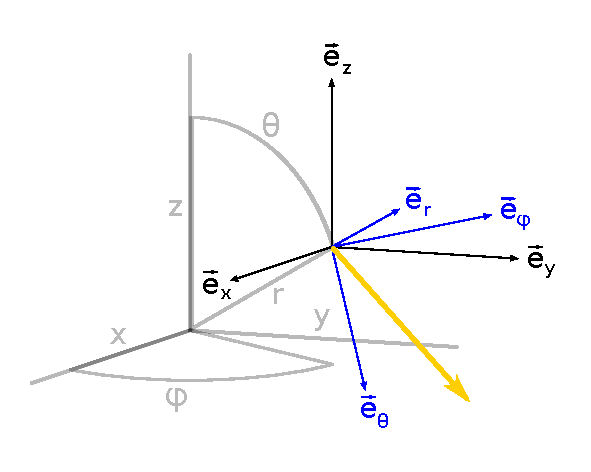
\includegraphics[width=1\linewidth]{Figures/spherical_polar_map}
  \end{subfigure}
  \begin{subfigure}{.45\textwidth}
    \centering
    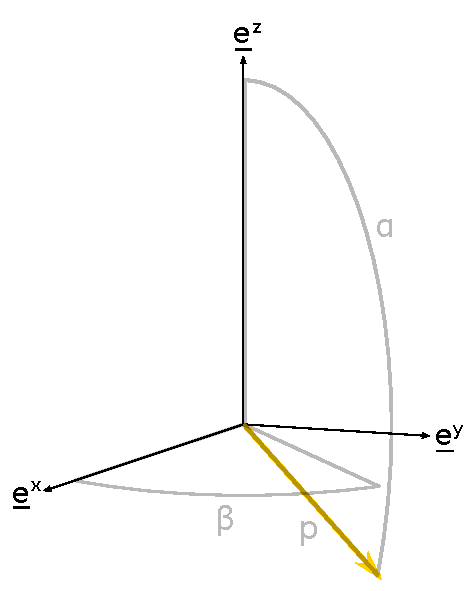
\includegraphics[width=0.8\linewidth]{Figures/neutrino_momentum_conventions}
  \end{subfigure}
  \caption[Conventions for momentum components]{
    In both diagrams, the broad yellow arrow represents the neutrino's momentum.
    \emph{Left Figure}:
    Spatial basis vectors ($\vec{e}_i\equiv\partial/\partial x^i$)
    at a representative position on the manifold.
    The coordinates $\{r,\theta,\phi\}$ are defined with respect to
    $\{x,y,z\}$ by the standard spherical polar to cartesian map
    (e.g.\ $x=r\sin\theta\cos\phi$).
    The spherical basis vectors are blue, and the cartesian basis vectors black.
    \emph{Right Figure}:
    The cotangent space at the neutrino's position.
    The neutrino momentum 1-form, $p_\mu$,
    may be written componentwise using the basis dual to $\vec{e}_i$
    ($\underline{e}^i\equiv dx^i$).
    The neutrino momentum is completely specified by three numbers.
    We use $\{p_t$,$\alpha$,$\beta\}$, which describe the cartesian spatial
    components of $p_\mu$ with the standard spherical polar to cartesian map
    (e.g.\ $p_x=p\sin\alpha\cos\beta$).
    The $p$ in these formulae is the Euclidean magnitude,
    $p = (p_x^2+p_y^2+p_z^2)^{1/2}$, related to $p_t$ by
    Eqns.~\ref{eqn:p_to_pt}~and~\ref{eqn:angular_factor}.
    (Note, we draw the neutrino's momentum vector embedded in the
    spatial manifold in the left figure, even though it properly lives only in
    the cotangent space in the right figure.)
    }
  \label{fig:p_conventions}
\end{figure}

To clean up some future calculations, we also define a 1-form on the
spatial manifold, $\Omega_i$, so that
\begin{align}
  &\Omega_i :\equiv (\sin \alpha \cos \beta, \sin \alpha \sin \beta, \cos \alpha) \\
  &p_i = p\,\Omega_i.
\end{align}

The fourth component of the momentum is constrained by the null condition,
$0=\psi^{\mu\gamma}p_\mu p_\gamma$.
In the 3+1 foliation of spacetime, we have
\begin{equation}
  \psi^{\mu\gamma}p_\mu p_\gamma
  = -\frac{1}{\alpha^2} p_t^2 + \frac{2}{\alpha^2} \beta^i \Omega_i p\, p_t
  + (g^{ij}-\frac{\beta^i \beta^j}{\alpha^2}) \Omega_i \Omega_j p^2, \nonumber
\end{equation}
whose solution is
\begin{equation}
  \label{eqn:p_to_pt}
  p_t = C(\Omega_i) \, p
\end{equation}
\begin{equation}
  \label{eqn:angular_factor}
  C(\Omega_i) \equiv \beta^i \Omega_i \pm
  \alpha \sqrt{g^{ij} \Omega_i \Omega_j}.
\end{equation}

As a check it is easy to confirm that for
$\psi_{\mu \nu}=\eta_{\mu \nu}:=\text{diag}(-1,1,1,1)$,
$C \rightarrow -1$, recovering the flat space connection between time and space
components of momentum. This check also confirms that we use the minus sign in
Eqn.~\ref{eqn:angular_factor}.

In some cases I will break from this convention with a simple rotation, in order
to have a momentum basis oriented with respect to the radial direcion, $\hat{r}$.
I label momentum colatitude and azimuthal angles in the rotated frame as $A$
and $B$ respectively. These angles are related to $\alpha$ and $\beta$ by a
simple Euler rotation, the specifics of which are irrelevant to this thesis.

\subsection{Numerical Integration}
\label{ssec:timestepping}
Eqns.~\ref{eqn:geo_x}--\ref{eqn:geo_tau} are solved by discretizing time and
performing a numerical integration.
I describe that process here.

A first-order ordinary differential equation has the form
\begin{equation}
  \partial_t u = L(u),
\end{equation}
which may be discretized into timesteps.
The value of $u$ at the $n$-th timestep is updated to its value
$\Delta t$ later by a fifth-order-accurate Dormand-Prince algorithm,
represented here abstractly as DP5[...]:
\todo{cite?}
\begin{equation}
  u^{n+1} = {\rm DP5}[L,u^n,\Delta t].
\end{equation}

As a high-order integration method, DP5 consists of a series of sub-steps.
Each sub-step evaluates the equation's right hand side, $L(u)$, using $u$ from
the previous step.
\todo{also dense output}
DP5 is an embedded Runge-Kutta algorithm, designed to also yield
a fourth-order-accurate solution with few additional evaluations of $L(u)$.
The difference in $u^{n+1}$ between the fourth- and fifth-order-accurate
solutions gives an estimate of the error for that step size. If this error is
larger than some threshold, we reduce the timestep, and try again from $u^n$.
\todo{Abs-Rel explicit}

The DP5 algorithm works as well for a system of coupled equations,
like the seven components of Eqns.~\ref{eqn:geo_x}--\ref{eqn:geo_tau}:
$\{x^x,x^y,x^z,p_x,p_y,p_z,\tau\}$.
In this case, the above prescription holds, but we think of $u$ as a
vector and $L$ as a vector-valued vector function.

We terminate the ray at the neutrinosurface, where $\tau=1$.
However, because a priori we do not know how much optical depth will accumulate
over a given timestep, we simply overstep the neutrinosurface, terminating at
the step N for which $\tau^{N-1}<1$ and $\tau^N\geq1$. Using the DP5 sub-steps
to interpolate $\tau$ to any time between $t^{N-1}$ and $t^{N}$, we search
this domain for the time $t_0$ that solves the equation
$\tau(t)=1$, using a robust Newton-Raphson root finding algorithm.
\todo{expected convergence order}
We examine the error associated with the uncertainty in the location of the
neutrinosurface in Sec.~\ref{sssc:af_sphere}.

\subsection{Code Tests}
\label{ssec:f_tests}
To test our code, we compute $f$ in two scenarios for which the analytic solution
is known.

\subsubsection{Homogeneous Minkowski}
In a homogeneous medium of temperature $T$, opacity $\zeta$, and neutrino chemical
potential $\eta$, on a flat spacetime manifold, $f$ is isotropic and homogeneous:
\begin{equation}
  f(x^\alpha;p_k) \rightarrow f(\varepsilon)
  =(e^{\varepsilon/k_{\rm B}T-\eta}+1)^{-1}
\end{equation}
The solution is scale-invariant because the observer sits inside of a
neutrinosurface which emits the same number of neutrinos per angle per energy
whether the surface is near (for high-energy rays) or far (for low-energy rays).

Despite this scale-invariance, we may calculate the length of a ray of energy
$\varepsilon=-p_t=p^t$ from Eqn.~\ref{eqn:geo_tau}:
$\ell \equiv c\Delta t = \Delta \tau/\zeta\varepsilon^2$, in order to test the
opacity integration by ray tracing code.

In our code test, we used volume data:
$T=5$~MeV,
$\zeta_{\nu_i}=\{0.01,0.005,0.001\}$~km$^{-1}$~MeV$^{-2}$, and
$\eta_{\nu_i}=\{0.1,-0.1,0\}$.
We sampled the distribution functions by tracing rays of energy
$\varepsilon=10$~MeV, and found neutrinosurfaces at distances of
$\ell_{\nu_i}=\{2.00,1.00,10.0\}$~km and neutrino number densities of
$f_{\nu_i}=\{0.109,0.130,0.119\}$ for each species respectively,
as expected. These results were exact to double precision because the fields
varied smoothly, and interpolation was exact.

\subsubsection{Asano-Fukuyama Sphere}
\label{sssc:af_sphere}
Outside of a hot, compact, non-rotating star in dynamical equilibrium, the
spacetime is spherically symmetric and stationary. The only solution of that
kind satisfying Einstein's equations is the Schwarzschild spacetime.
In Schwarzschild spherical polar coordinates, the metric takes the form
$\psi_{\mu\gamma}(r):={\rm diag}\left(-\alpha^2(r),\alpha^{-2}(r),r^2,r^2\sin^2\theta\right)$,
where the lapse is $\alpha(r)=(1-R_g/r)^{1/2}$, and the gravitating mass is
$M=R_g/2$.
(Note, this scenario was examined semi-analytically by Asano and Fukuyama (2000),
\todo{cite properly}
to estimate the neutrino-antineutrino annihilation power outside of a collapsed
stellar core.)

A neutrino is emitted from the neutrinosphere at $R_\nu$, with energy
$\varepsilon'$ in the fluid rest frame.
%(with $u^\beta:=(-\alpha(R_\nu),0,0,0)$, so that
%$p_{\nu t}=-\alpha(R_\nu)\varepsilon'$),
It will be measured by a stationary observer at $r$
%(for whom $U^\beta:=(-\alpha(r),0,0,0)$),
as having a lower energy
$\varepsilon=\varepsilon' \, \alpha(R_\nu)/\alpha(r)$.
Therefore, for momentum angles in the direction of the neutrinosphere,
$f(\varepsilon)=\left(\exp(\varepsilon/k_{\rm B}T_{\rm eff}-\eta)+1\right)^{1/2}$,
with an effective temperature $T_{\rm eff}=T \, \alpha(R_\nu)/\alpha(r)$,
where $T$ is the fluid temperature measured in the fluid rest frame.
In terms of the conventional momentum variables $\{p_t,\alpha,\beta\}$
introduced in Sec.~\ref{ssec:p_conventions}, we have
\begin{equation}
  \label{eqn:asano_fukuyama_f}
  f(x^\alpha;p_k) \rightarrow f(r;p_t,A)
  =\left\{
  \begin{matrix}
    (e^{-p_t/k_{\rm B}T\sqrt{(1-R_g/R_\nu)}-\eta}+1)^{-1} & A \leq A_{\rm max}(r) \\
    0                                                            & A > A_{\rm max}(r)
  \end{matrix}
  \right.
\end{equation}
where $A$ is the angle $p_k$ makes with a radial ray, and
$A_{\rm max}$ is the half-angular size of the star as viewed from $r$.
In a flat spacetime it's simple: $\sin A_{\rm max} = R_\nu/r$.
But in the Schwarzschild spacetime, where neutrino trajectories bend around the
star,
\begin{equation}
  \label{eqn:angular_extent}
  \sin A_{\rm max} = \frac{R_\nu}{r} \sqrt{\frac{1-R_g/r}{1-R_g/R_\nu}},
\end{equation}
as derived by Asano-Fukuyama (2000).
\todo{cite properly, and fix, this isn't your angle $A$}

Fig.~\ref{fig:f_hot_ns} shows $f(p_t=20\,{\rm MeV})$ across all angles for
a patch of sky centered on the emitter. The spacetime and the emitter are
characterized by $T=5$~MeV, $\eta=0.1$, $R_g=2\,M_\odot$, $R_\nu=3\,M_\odot$.
To impose a sharp neutrinosphere at $R_\nu$, we use a step function opacity
with $\zeta=10^6\,{\rm Msun}^{-1}\,{\rm MeV}^{-2}$ inside the star.
This scenario represents an unphysically compact star (in fact, this
neutrinosphere coincides with the radius of circular neutrino orbits), but it
serves its purpose here to stress-test the ray tracing code in strong gravity.
For comparison, in the same figure we also show a ray-tracing sampling of $f$
at the same coordinate viewing position for the same star embedded in flatspace.
Both the angular extent of the stars in Fig.~\ref{fig:f_hot_ns}, and the
intensity of neutrinos emitted by their surfaces at this energy agree
with the analytical predictions given by
Eqns.~\ref{eqn:angular_extent}~and~\ref{eqn:asano_fukuyama_f}.

For this test we use a fixed timestep, $\Delta t = 0.2\,M_\odot$,
because the adaptive timestepper described in Sec.~\ref{ssec:timestepping} is
not very effective with discontinuous fields, like $\zeta$. In physical
fluid configurations, we expect to encounter discontinuities also (though
probably not as extreme), and we may have to used fixed timesteps in those
cases also.

In Fig.~\ref{fig:f_hot_ns}, the Schwarzschild case, the variation in $f$
across the surface of the star is a spurious artifact of our finite timestep:
the redshift is greater along directions whose rays yield an estimate of the
neutrinosurface at $r<R_\nu$, and lesser for neutrinosurfaces at $r>R_\nu$.

\begin{figure}
  \centering
  \begin{subfigure}{.8\textwidth}
    \centering
    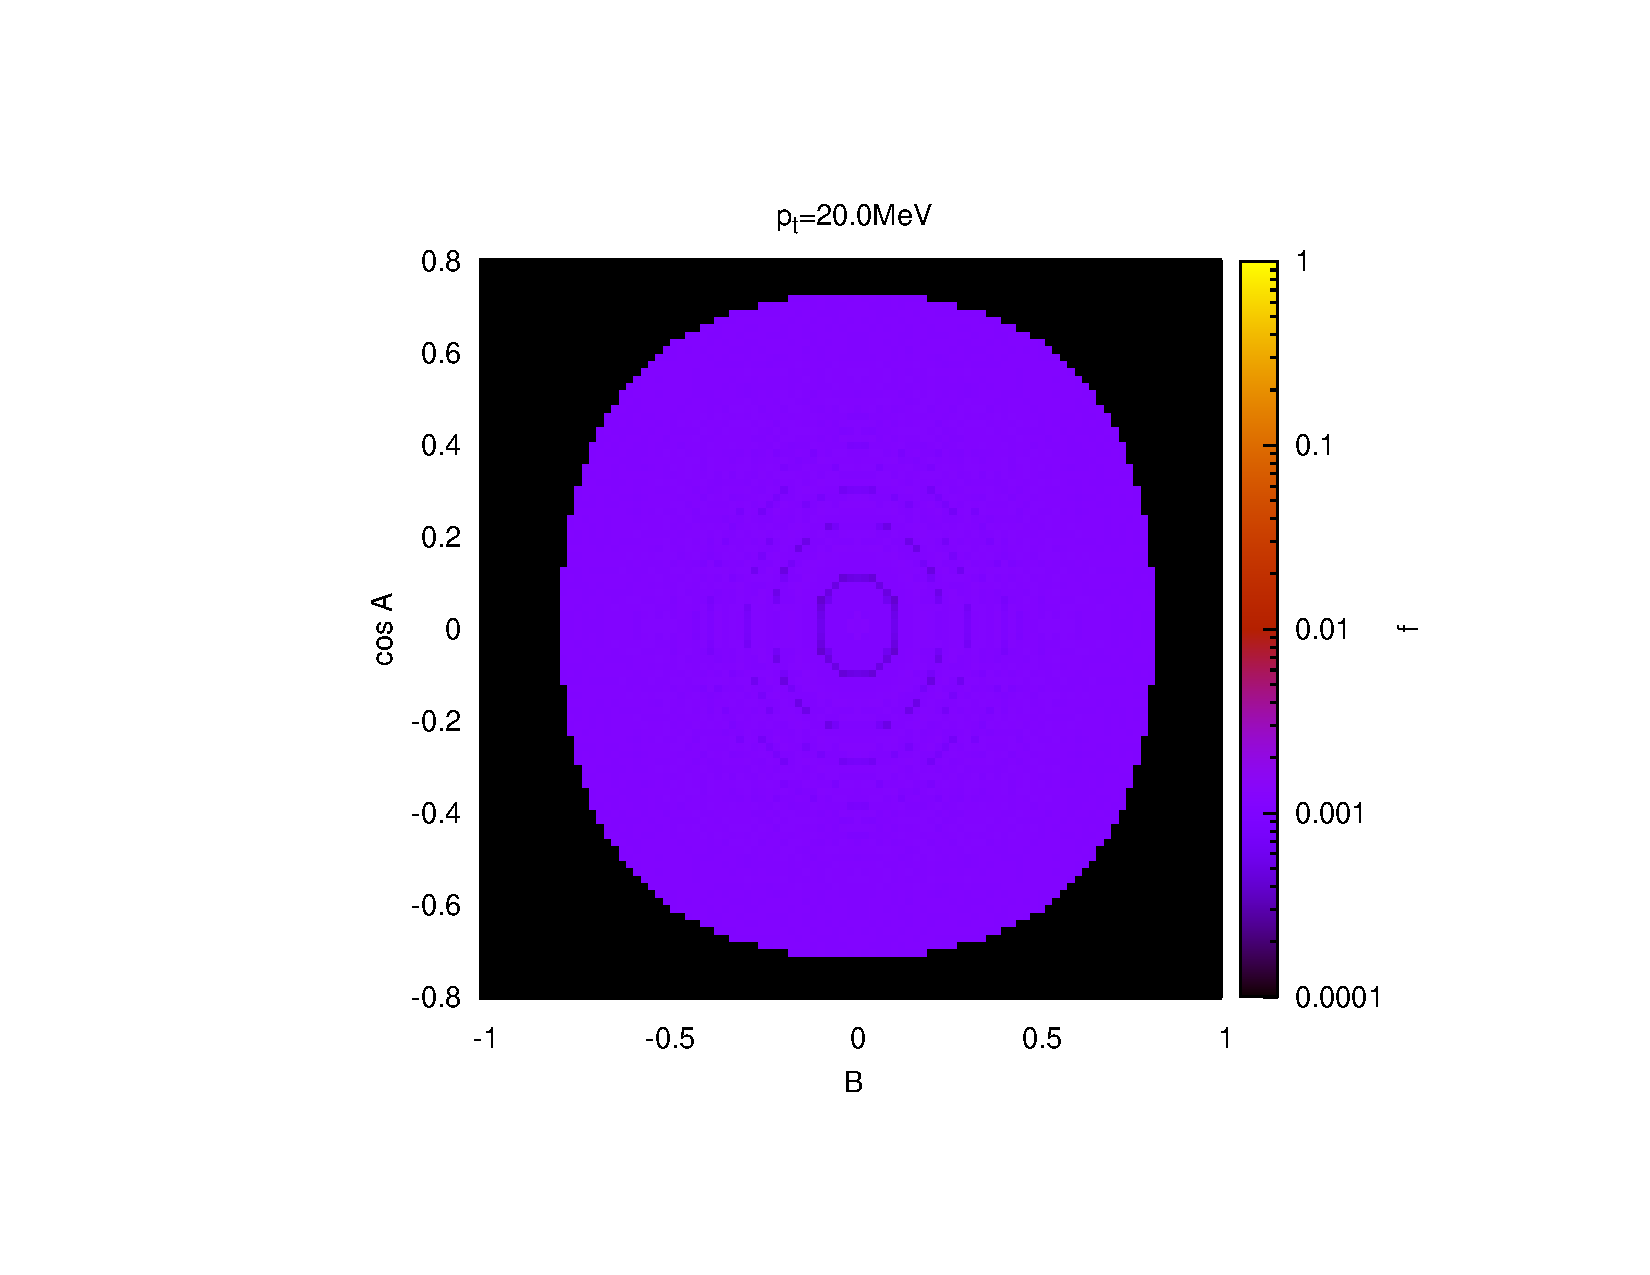
\includegraphics[width=1\linewidth]{Figures/fnue_Alpha_vs_Beta-asano_fukuyama_gr}
  \end{subfigure}
  \begin{subfigure}{.8\textwidth}
    \centering
    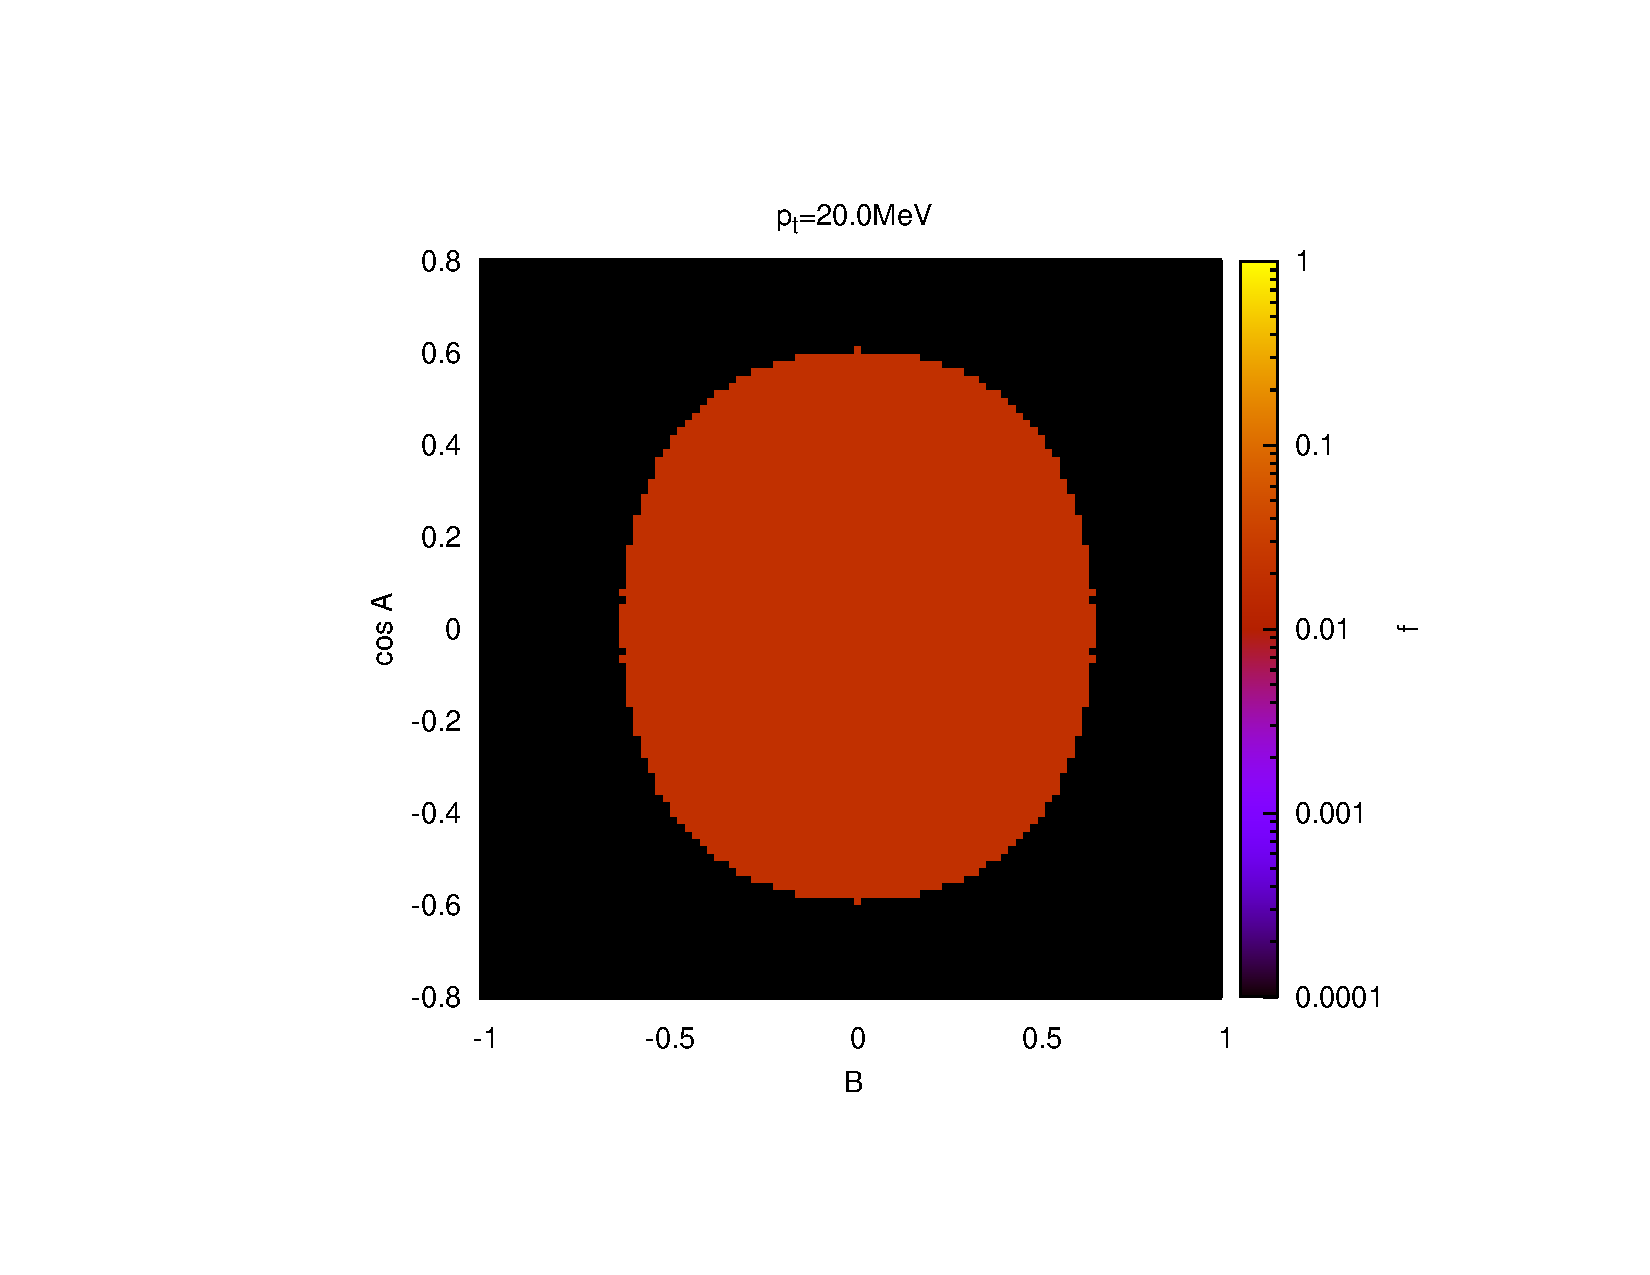
\includegraphics[width=1\linewidth]{Figures/fnue_Alpha_vs_Beta-asano_fukuyama_flat}
  \end{subfigure}
  \caption[Monochromatic sky map of $f$ for the hot compact star]{
    $f$ across a patch of sky in a single energy band, $p_t=20$~MeV.
    The source is a hot compact star: $R_g=2\,M_\odot$, $R_\nu=3\,M_\odot$,
    $T=5$~MeV, and $\eta=0.1$.
    The observer is stationary at Schwarzschild radius $5\,M_\odot$.
    \emph{Top Figure}: Schwarzschild spacetime.
    \emph{Bottom Figure}: Minkowski spacetime.
    These two stars have identical coordinate radii, and identical local fluid
    properties at their neutrinospheres.
  }
  \label{fig:f_hot_ns}
\end{figure}

Fig.~\ref{fig:f_spectrum_hot_ns} presents the energy spectrum emitted by this
surface over the broad band $p_t\in[0.01,100]~MeV$, for both Schwarzschild
and Minkowski cases.
We also show the relative errors in $f(p_t)$, with respect to the analytic
solution $f_{\rm ex}(p_t)$. The Minkowski calculation is exact to machine
precision, because location of the neutrinosurface has no effect on $f$.
But the relative errors in the Schwarzschild case are large, and grow to
20\% at 100~MeV. (It is important to keep in mind that this is not the case
generally, but only when the neutrinosurface is in a steep gravitational
potential.
This will be an important consideration in Sec.~\ref{sec:q_algorithm}:
spectral information at energies near 100~MeV can be important in the
neutrino-antineutrino annihlation calculation because the process depends very
steeply upon the neutrino energies.

\begin{figure}
  \centering
  \begin{subfigure}{.7\textwidth}
    \centering
    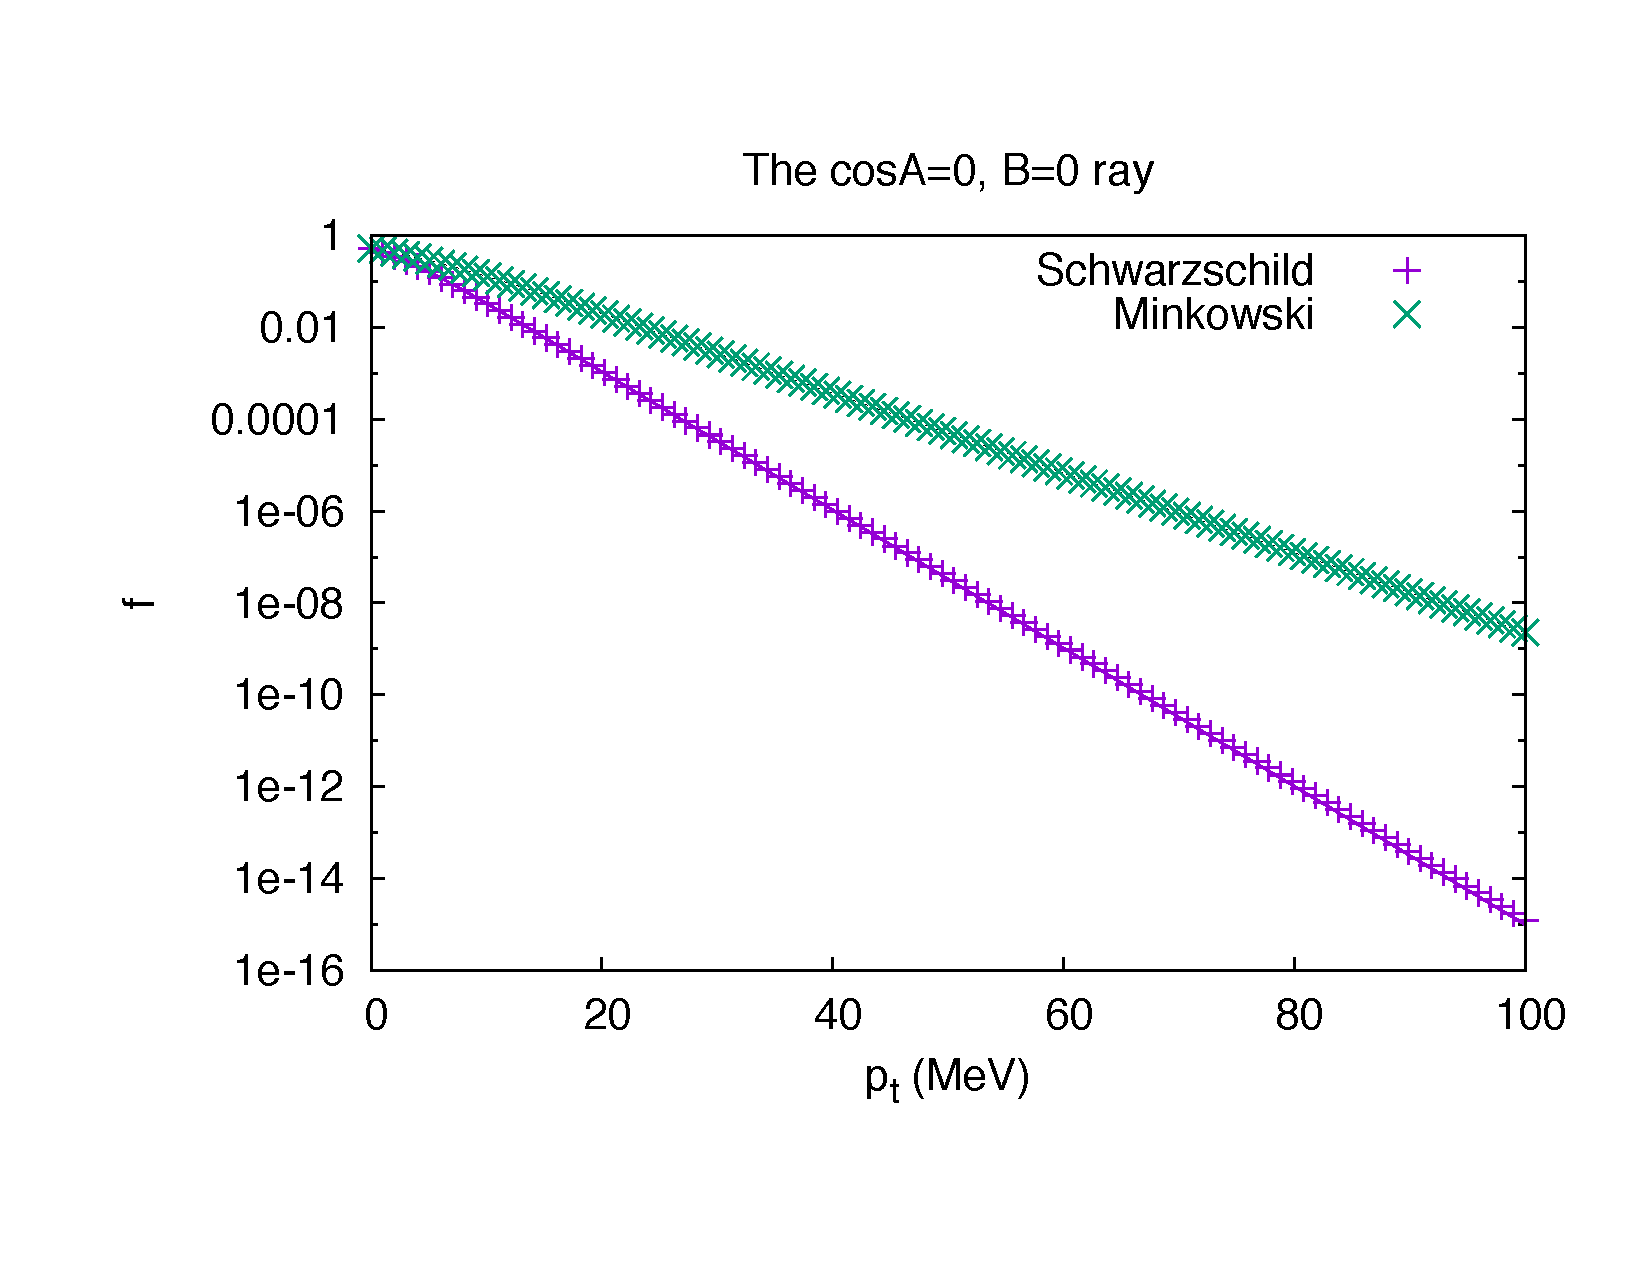
\includegraphics[width=1\linewidth]{Figures/fnue_vs_E-asano_fukuyama}
  \end{subfigure}
  \begin{subfigure}{.7\textwidth}
    \centering
    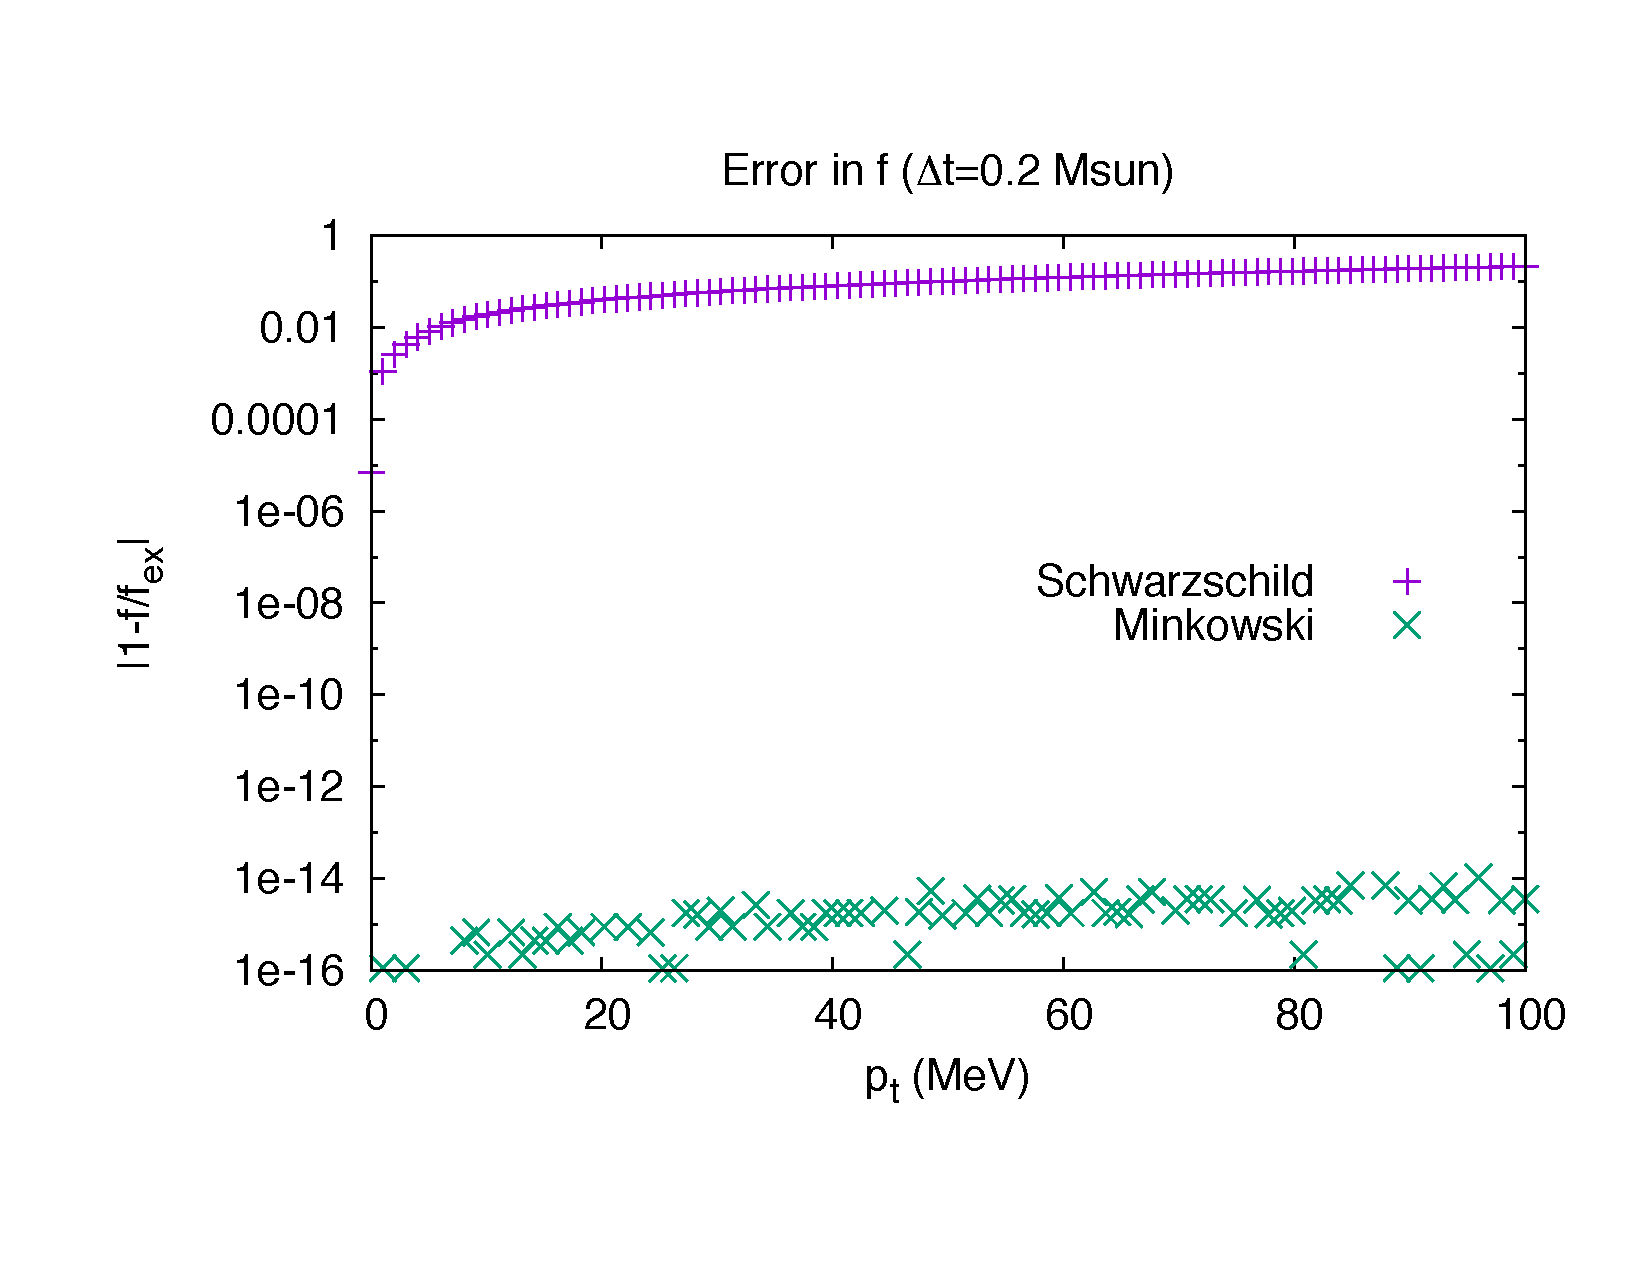
\includegraphics[width=1\linewidth]{Figures/fnueError_vs_E-asano_fukuyama}
  \end{subfigure}
  \caption[Asymptotic energy spectrum of the hot compact star]{
    The $p_t$ spectrum of the hot compact star from the same viewing
    position as in Fig.~\ref{fig:f_hot_ns}. These plots show $f$ sampled by
    the $\cos A=0$, $B=0$ rays.
    \emph{Top Figure}: $f(p_t)$ in the case of a curved and flat spacetime.
    The exact distribution functions $f_{\rm ex}$ are represented as solid lines,
    which lie directly beneath the data points.
    \emph{Bottom Figure}: The relative error in $f$ for these two cases.
    For the flat spacetime distribution function, the error bottoms out at
    machine roundoff.
  }
  \label{fig:f_spectrum_hot_ns}
\end{figure}

\section{$f_\nu$ for this Accretion Disk}
\label{sec:f_this_case}

\section{Calculating $q_{\nu \bar{\nu}}$: Integration Algorithm}
\label{sec:q_algorithm}

\section{$q_{\nu \bar{\nu}}$ for this Accretion Disk}
\label{sec:q_this_case}
